\section{Theoretical Introduction}
\label{sec:theoretical}


\paragraph{}When it comes to this amplifier, it is exactly of the same type of the first one mentioned in the introduction, it is the circuit of a speaker. As such, the objective of this lab assignment is to build a circuit that has an input source of  $10mV$ and an output speaker of $8\Omega$.

\paragraph{}In very broad terms, this circuit is going to be divided in two: a gain stage that will amplify the input sound signal as much as possible and an output stage, which will make the amplifier's output impedance compatible with impedance of the speaker.  

\begin{figure}[h] \centering
	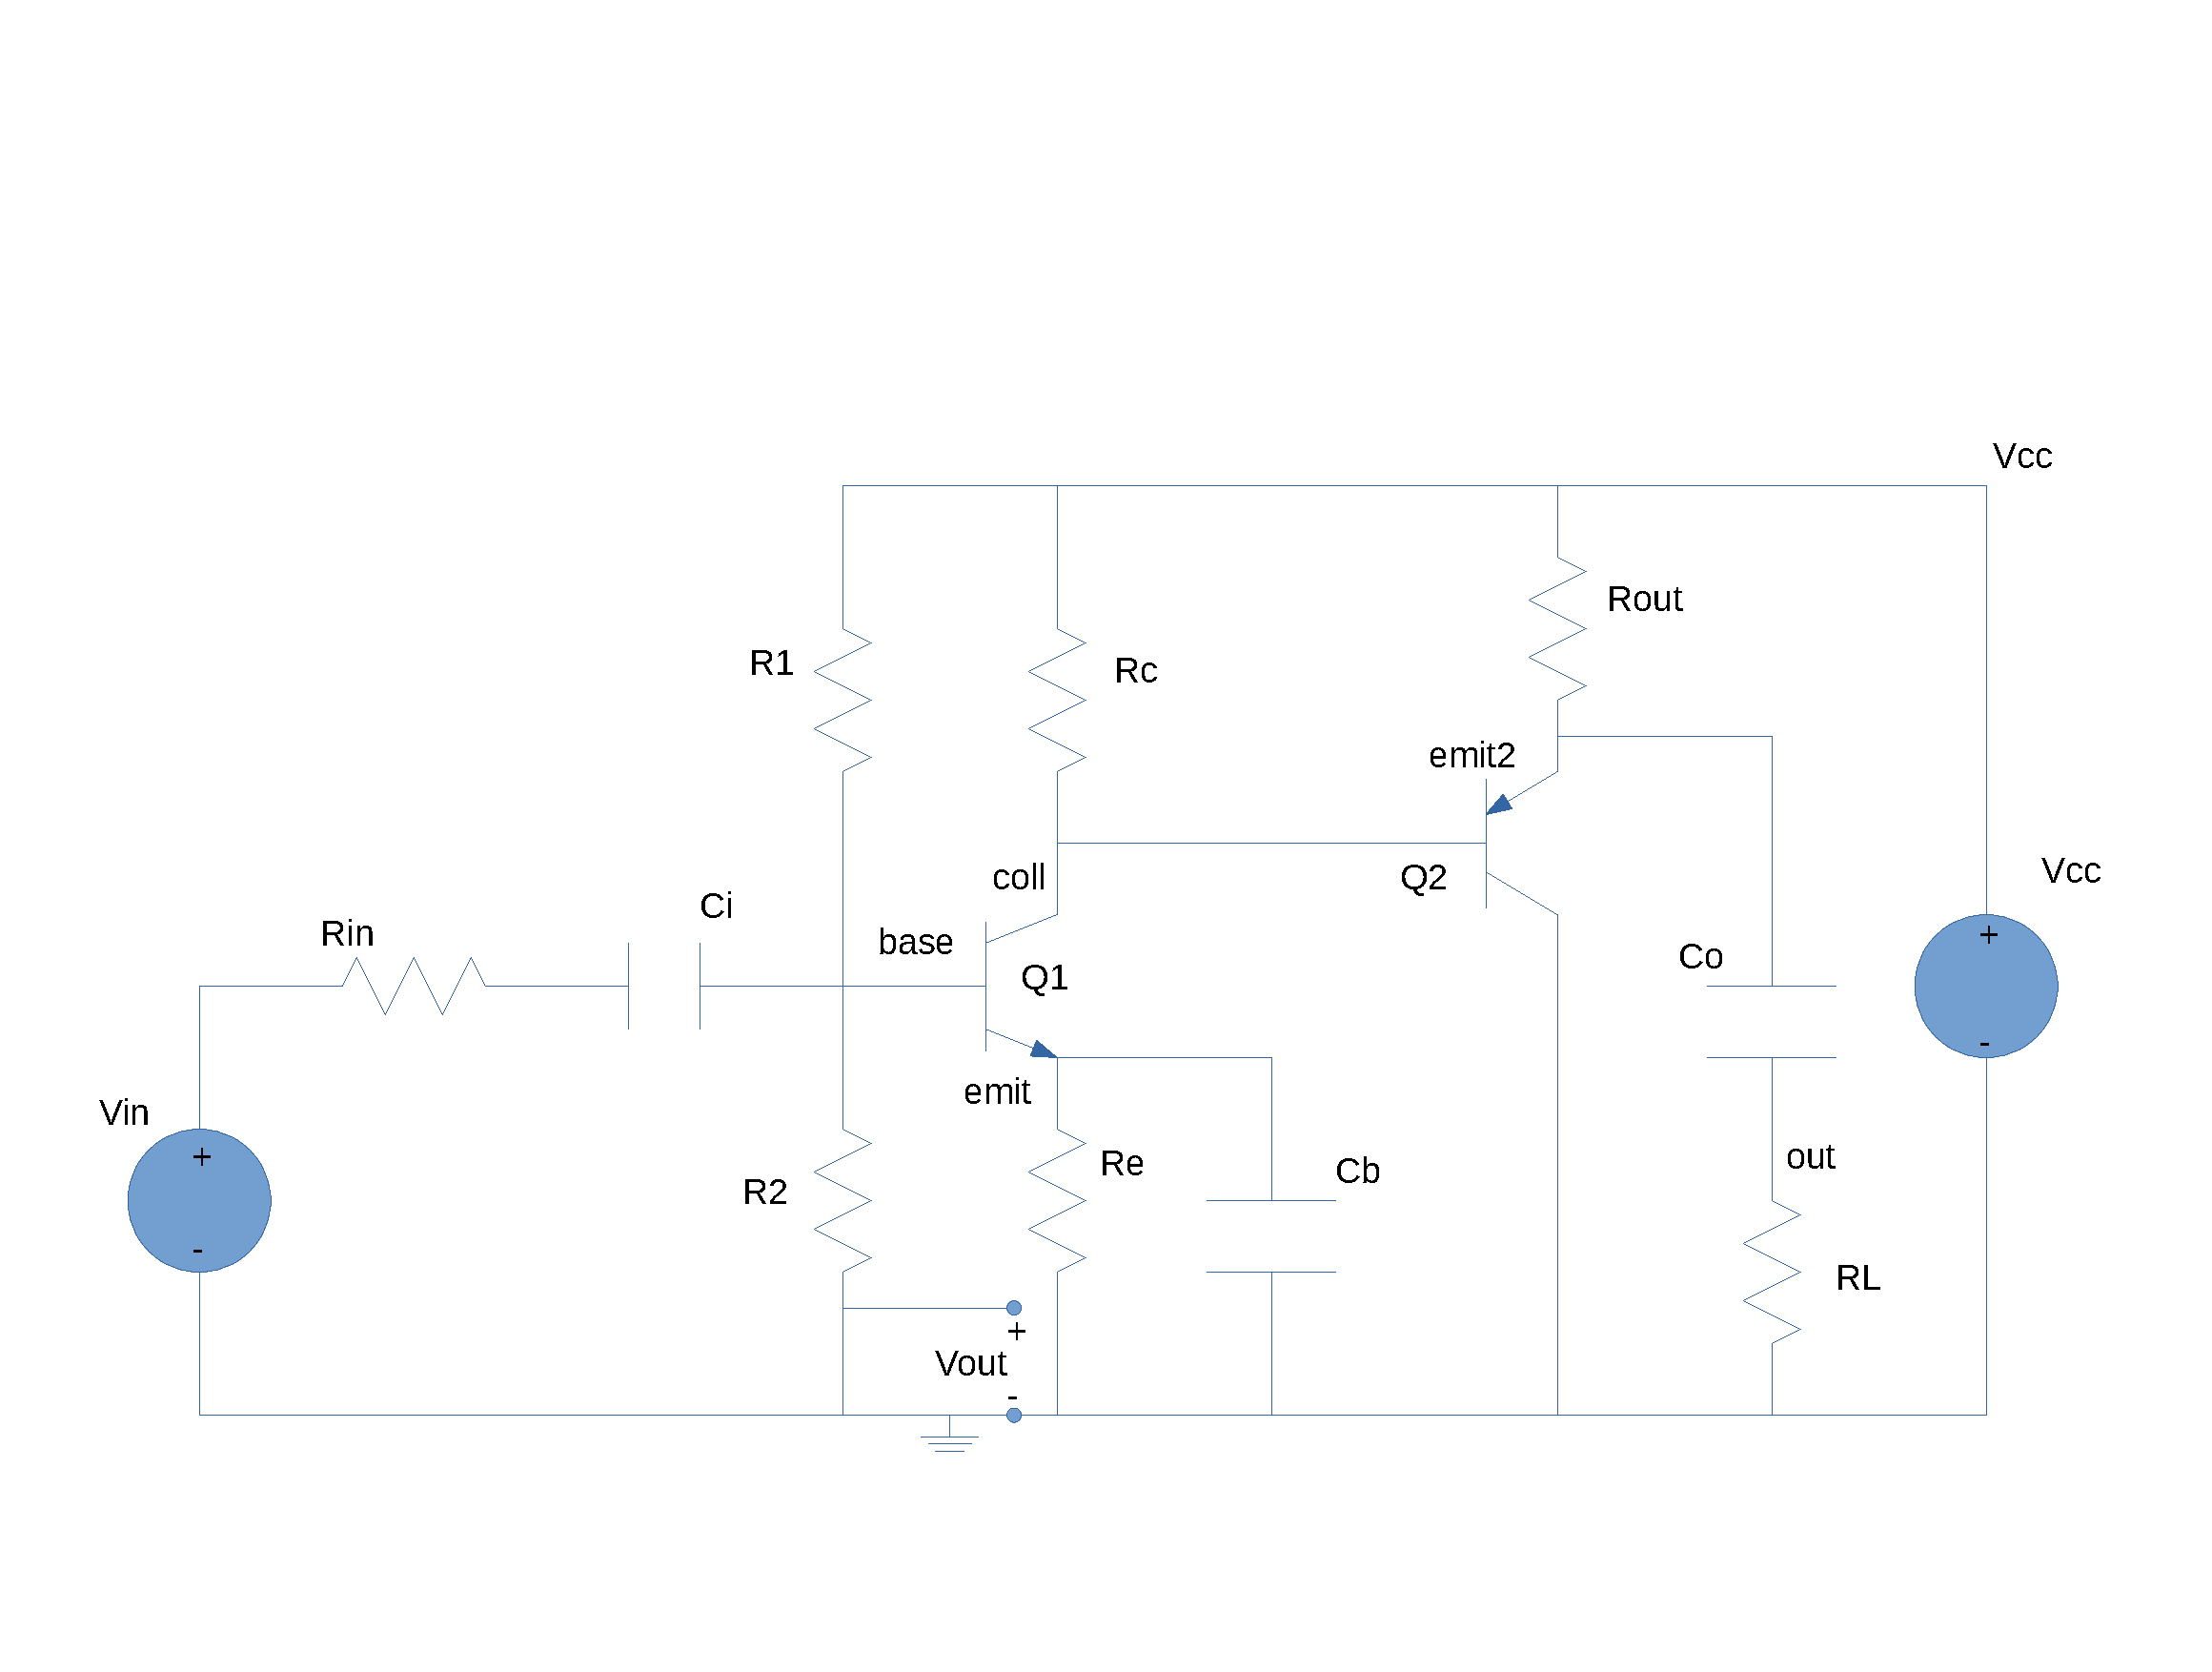
\includegraphics[width=0.8\linewidth]{circuit.pdf}
	\caption{Fourth laboratory circuit.}
	\label{fig:circuit}
\end{figure}


